\documentclass[review,12pt]{elsarticle}

%% ---- page style patch: avoids elsarticle preprint-footer overfull box ----
\makeatletter
\def\ps@pprintTitle{%
  \let\@oddhead\@empty\let\@evenhead\@empty
  \def\@oddfoot{\footnotesize\hfill\thepage\hfill}%
  \let\@evenfoot\@oddfoot}
\makeatother

\usepackage{amsmath}
\usepackage{booktabs}
\usepackage{graphicx}
\usepackage{tabularx}
\usepackage{adjustbox}
\usepackage{xcolor}
\usepackage[
  colorlinks=true,
  linkcolor=blue,
  citecolor=darkgray,
  urlcolor=blue,
  bookmarks=true,
  bookmarksnumbered=true,
  unicode=true
]{hyperref}

\usepackage{natbib}
\bibliographystyle{elsarticle-num}

\setlength{\parskip}{0pt}

\begin{document}

\begin{frontmatter}

\title{Free and Fair? A Systematic Study of Reliability and Bias
       in Open-Source LLM Judges across Families and Scales}

\author[dlut]{Chang Tan}
\address[dlut]{Dalian University of Technology, Dalian 116024, China}

\begin{abstract}
Free-tier LLM APIs make large-language-model judges accessible to any
budget, yet the reliability of these freely usable referees is largely
uncharacterised. We audit ten open-source judges from four model families
(Qwen, DeepSeek, GLM, Kimi) plus two proprietary free-tier references
under one protocol: 400 answer pairs spanning mathematics, factual QA,
creative writing, and abstract explanation, each judged in both
presentation orders, with a test--retest subset and ground-truth-controlled
family-preference probes, all at zero monetary cost. Four findings stand
out. First, severity collapse: DeepSeek flash and flagship judges abstain
with ties on 50--59\% of pairs, dragging their ground-truth accuracy as
low as 0.32. Second, instruction backfire: a standard anti-verbosity
sentence inverts the usual verbosity bias, producing significant
preference for the \emph{shorter} answer ($-0.46$ log-odds per 1{,}000
characters). Third, family-specific kinship: Qwen judges significantly
avoid same-family answers while GLM and Kimi reward them even when the
reference answer proves them wrong. Fourth, panel gains without
debiasing: majority voting over three judges raises ground-truth
accuracy from 0.58 to 0.85 but leaves the shared position-bias component
essentially unchanged, so order swapping remains necessary. We distill the
results into six deployment guidelines and release the complete
artifact---questions, prompts, 9,453 verdicts, and analysis code---so the
audit can be re-run as free-tier catalogues evolve.
\end{abstract}

\begin{keyword}
LLM-as-a-Judge \sep evaluation reliability \sep position bias \sep
self-preference bias \sep open-source models
\end{keyword}

\end{frontmatter}

%% ==================================================================
\section{Introduction}
\label{sec:intro}

Large language models (LLMs) are increasingly asked not only to produce
answers but also to grade them. The LLM-as-a-Judge paradigm, in which a model
compares or scores candidate responses in place of human annotators, has
become a workhorse of modern language technology. It powers public leaderboards
built on pairwise comparison \citep{zheng2023judging}, substitutes for human
preference labels in instruction tuning pipelines, and provides cheap
regression tests for retrieval-augmented systems, agents, and text generation
services \citep{liu2023geval,gu2024survey}. As the scale of evaluation grows
far beyond what human rating budgets can cover, the quality of machine
judgement itself has become a first-order scientific question.

The dominant practice rests on a small set of closed, frontier models such as
GPT-4 and Claude. This reliance carries well-known costs: per-token fees that
grow linearly with evaluation volume, restricted data governance, and
reproducibility risks when a provider silently updates a checkpoint. Open
models offer an appealing alternative. Their weights are public or freely
hosted, and several providers expose capable open families through zero-cost
API tiers, which makes them attractive to academic groups and small
engineering teams. Whether these freely accessible models can actually serve
as dependable judges, however, remains poorly characterized. Existing bias
studies concentrate on closed judges from a handful of providers
\citep{zheng2023judging,chen2024humans,norman2026reliability}, and the
largest recent audit of 21 judges covers nine commercial providers while
leaving open-weight families at the periphery. Openness does not imply
neutrality: a judge trained by the same organization that produced some of the
candidates may share stylistic priors, tokenization habits, or even training
data with those candidates, which creates a structural risk of family
favoritism that earlier self-recognition studies only partially capture
\citep{panickssery2024llm}.

This paper presents a systematic anatomy of reliability and bias for
freely accessible LLM judges. We assemble ten open-source judges drawn from
four model families (Qwen, DeepSeek, GLM, and Kimi), spanning multiple
capability tiers within each family, and complement them with two proprietary
free-tier judges (Agnes-2.5-Flash and Agnes-3.0-Flash) as a reference group,
evaluating all of them under one unified protocol. Five generators, one per
family plus a second Qwen tier, answer 200
questions from four domains: grade-school mathematics with verifiable ground
truth \citep{cobbe2021training}, adversarial factual QA with reference answers
\citep{lin2022truthfulqa}, open-ended creative writing, and abstract
explanation. From these answers we construct 400 stratified answer pairs, and
every judge scores every pair in both presentation orders, yielding
9,453 usable verdicts, with an additional test-retest subset of
640 repeated judgements on the open judges to probe stochastic
stability.

The design isolates four bias families with matched measurements for every
judge. Position bias is measured directly by comparing verdicts on swapped
presentation orders, length bias by the conditional win rate of the longer
answer, accuracy on ground-truth-clear pairs in the two verifiable domains,
and family preference by a quality-controlled protocol that tracks how often
a judge rewards a same-family answer when the reference answer proves that
answer wrong. Inter-judge structure is summarized by pairwise Cohen's kappa
\citep{cohen1960coefficient}, and all headline estimates carry question-level
cluster bootstrap confidence intervals.

Four findings structure the results. \emph{Severity collapse}: the
DeepSeek flash and flagship judges return ties on 50--59\% of pairs,
silencing their discrimination and pushing ground-truth accuracy below
chance, a failure mode invisible to compliance checks. \emph{Instruction
backfire}: the standard anti-verbosity rubric sentence inverts the usual
verbosity bias---every Qwen, GLM, and Kimi judge tilts against the longer
answer, significantly so in the pooled regression. \emph{Lineage-specific
kinship}: Qwen judges avoid same-family answers (37\% kin win rate) while
GLM-5.3 and Kimi-K3 reward theirs even when the reference proves them wrong
(27--33\% kin-wrong pick rate). \emph{Panel gains without debiasing}:
majority voting over three free judges lifts accuracy from 0.58 to 0.85
while leaving the shared position-bias component essentially unchanged,
showing that panels are accuracy instruments, not debiasing ones.

Beyond measurement, we translate the findings into deployment guidance for
practitioners who cannot afford commercial judge APIs. We quantify how
majority panels of three or five open judges trade compute for accuracy and
bias robustness, revisit the order-swapping protocol as a cheap debiasing
device, and identify which free-tier models are safe to use as referees for
which kinds of tasks. All prompts, question sets, raw verdicts, and analysis
code are released with the paper to support reuse.

Our contributions are fourfold. First, we provide the first systematic,
multi-family, multi-tier study of judging reliability for freely accessible
LLM judges, covering four bias families under one protocol and contrasting
open-source judges with proprietary free-tier references. Second, we
introduce a quality-controlled kin-preference measurement that separates
family favoritism from genuine quality differences. Third, we give
within-family scale-gradient evidence that links judge behaviour to model
tier rather than to family identity alone. Fourth, we distill the results
into concrete, zero-cost judging guidelines and release the complete
experimental artifact.

%% ==================================================================
\section{Related Work}
\label{sec:related}

\subsection{LLM-as-a-Judge}
Using LLMs to evaluate text quality was popularized by G-Eval, which framed
NLG scoring as a probability-weighted form-filling task with chain-of-thought
\citep{liu2023geval}, and by MT-Bench, which established pairwise comparison
with a reference-guided rubric as the default protocol and reported the first
catalogue of judge failure modes \citep{zheng2023judging}. Subsequent surveys
systematized the design space of judges, prompts, and aggregation schemes
\citep{gu2024survey}. A complementary line of work trains open models
specifically for evaluation: the Prometheus family fine-tunes open LLMs on
human feedback to produce reproducible graders whose agreement with humans
rivals that of general-purpose judges \citep{kim2024prometheus}. Our study
differs in orientation: rather than proposing a new judge or benchmark, we
audit the judging behaviour of off-the-shelf open models that practitioners
can already call for free, since in practice most teams use unmodified
chat models as referees rather than dedicated evaluator checkpoints.

\subsection{Judgement Biases}
Three bias families dominate the literature. Position bias, the tendency to
favour whichever answer appears first (or last), was demonstrated early for
GPT-4-class judges and motivates order-swapping or consistency-based
mitigations \citep{zheng2023judging,wang2024fair,li2023split}. Verbosity bias,
the correlation between answer length and preference, was documented in RLHF
preference labels and in arena-style evaluation, and motivated
length-controlled win rates \citep{singhal2024long,dubois2024length}.
Self-preference is the subtler tendency of a judge to favour its own
generations: evaluators have been shown to recognize their own text and to
reward it, even when the text carries a hidden watermark that the judge
cannot consciously detect \citep{panickssery2024llm}. Comparative studies of
human and machine judges further show that some biases, such as
self-preference and conformity to anchor answers, are shared by humans and
LLMs, while others, such as opinionatedness, differ sharply
\citep{chen2024humans}. We generalize the self-preference lens from the
individual model to the model family: because several providers ship many
tiers of the same base model, a practical question is whether a judge favours
any member of its own lineage, which we measure with ground-truth controls.

\subsection{Reliability, Validity, and Judge Panels}
A growing body of work asks whether judges agree at all. Cross-judge
agreement with humans is often modest and task-dependent
\citep{hosking2023human,bavaresco2024llms}. A recent large-scale audit of 21
judges from nine providers reports that exact-match agreement overstates
discriminative ability relative to Cohen's kappa, that judge rankings are
unstable across benchmarks, and that high test-retest reliability can coexist
with severe position bias \citep{norman2026reliability}. Infrastructure work
such as JudgeArena unifies judge benchmarks and ships tuned configurations
for open judges \citep{lushtaku2026judgearena}. On the mitigation side,
panels of diverse judges have been proposed to average away idiosyncratic
errors \citep{verga2024replacing}, though correlated errors within panels can
undermine the diversity argument. Our contribution to this line is a
family-and-tier-resolved view of agreement structure among free judges, plus
a panel analysis that respects family boundaries, so that panel gains are not
confounded by kinship.

%% ==================================================================
\section{Experimental Setup}
\label{sec:setup}

\subsection{Model Roster}
\label{sec:roster}

Table~\ref{tab:roster} lists the twelve judges and five generators. The ten
open-source judges are served through a single OpenAI-compatible endpoint
(Alibaba Cloud Model Studio free tier) under identical API settings, which
removes serving differences as a confound. The open roster spans four
families: five Qwen checkpoints covering two flash generations, a 27B mid
tier, a max tier, and a 2.4T-parameter Mixture-of-Experts flagship
\citep{qwen2025qwen3}; three DeepSeek checkpoints covering two flash tiers
and a pro tier \citep{deepseek2024v3}; the GLM-5.3 flagship \citep{glm2024chatglm};
and Kimi-K3 \citep{kimi2025k2}. The same five
generators produce candidate answers, one flagship per family plus a second,
deliberately smaller Qwen tier so that within-family quality variance exists
for the kinship analysis. Two judges (Qwen3.8-2.4T and GLM-5.3)
are served with mandatory reasoning, a platform restriction of the free tier;
we account for this when interpreting their behaviour, and treat
\emph{thinking mode} as an observational variable rather than a confound to
be hidden.

Beyond the open roster, we add two proprietary judges, Agnes-2.5-Flash and
Agnes-3.0-Flash, accessed through their public API on the provider's
zero-priced promotional tier. These models give a proprietary reference
point against which the open judges can be read; they see the identical
judging prompt, but their serving platform injects undisclosed
system-level instructions ahead of it (observed as roughly 300--600 extra
prompt tokens per call), so their absolute metrics are indicative rather
than strictly comparable, a caveat we revisit in Section~\ref{sec:limitations}.

\begin{table}[t]
\centering
\small
\caption{Model roster. Judges evaluate all 400 answer pairs in both orders;
generators produce the candidate answers. Tier gives the capability level
within the family (F = flash/entry, M = mid, P = flagship/prime). Thinking
indicates whether the serving platform enables a reasoning phase that cannot
be disabled. Agnes judges are proprietary free-tier references (see text).}
\label{tab:roster}
\begin{tabular}{llllc}
\toprule
Model & Family & Tier & Role & Thinking \\
\midrule
Qwen3.7-Flash (0715)  & Qwen     & F & judge & no  \\
Qwen3.8-Flash         & Qwen     & F & judge + generator & no  \\
Qwen3.8-27B           & Qwen     & M & judge & no  \\
Qwen3.8-Max (0902)    & Qwen     & P & judge + generator & no  \\
Qwen3.8-2.4T-A95B     & Qwen     & P+ & judge & yes \\
\midrule
DeepSeek-V4-Flash (0731) & DeepSeek & F & judge & no  \\
DeepSeek-V4.1-Flash   & DeepSeek & F & judge & no  \\
DeepSeek-V4-Pro (0813)& DeepSeek & P & judge + generator & no  \\
\midrule
GLM-5.3               & GLM      & P & judge + generator & yes \\
Kimi-K3               & Kimi     & P & judge + generator & no  \\
\midrule
Agnes-2.5-Flash       & Agnes\textsuperscript{p} & F & judge & managed \\
Agnes-3.0-Flash       & Agnes\textsuperscript{p} & F+ & judge & managed \\
\bottomrule
\multicolumn{5}{l}{\footnotesize \textsuperscript{p}Proprietary judges, served via their own API.}
\end{tabular}
\end{table}

\begin{figure}[t]
\centering
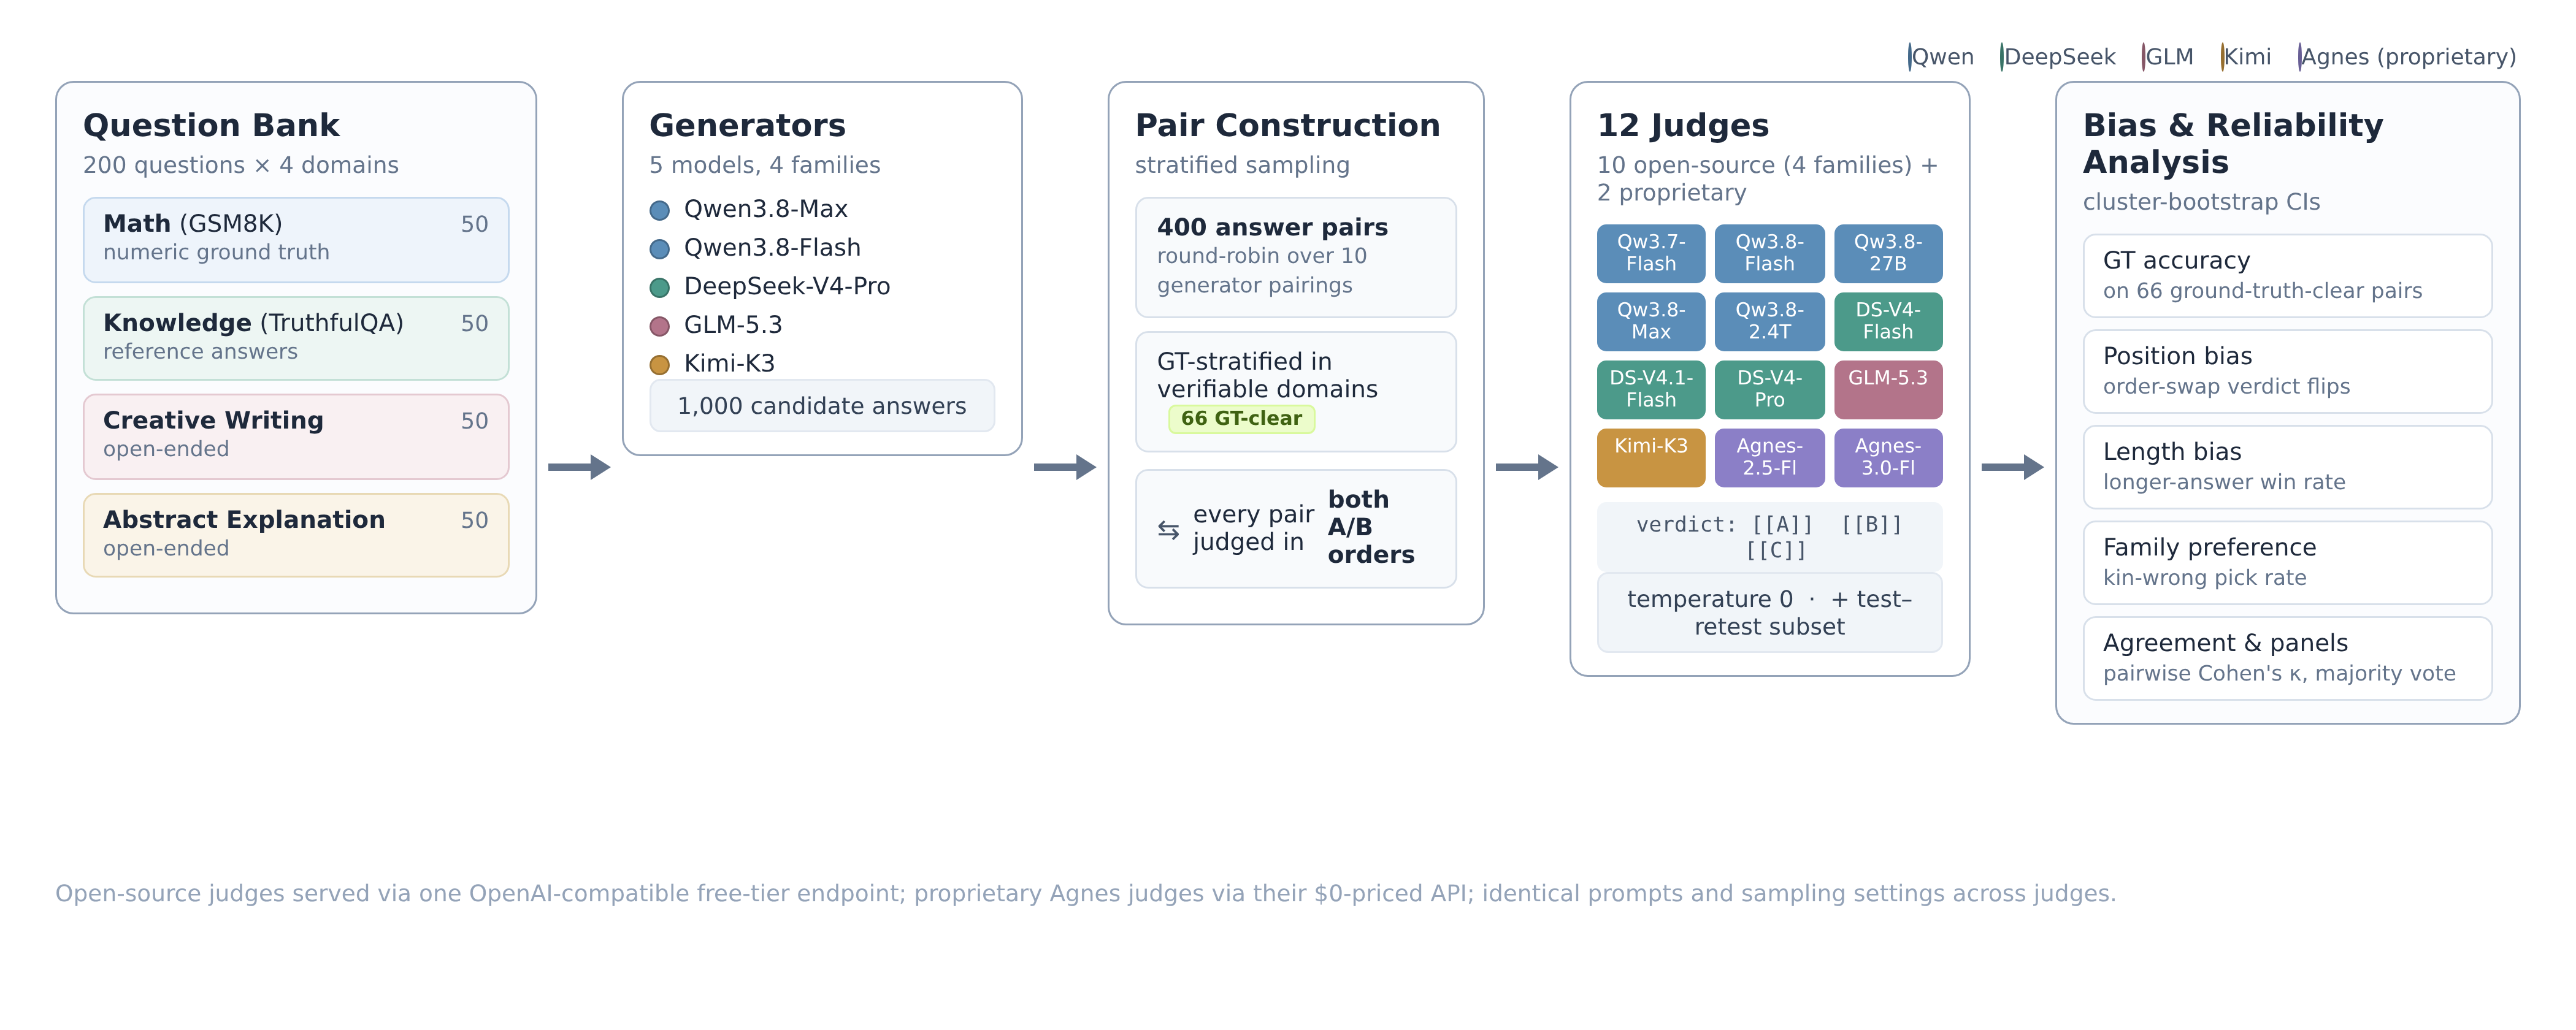
\includegraphics[width=\textwidth]{figures/fig_framework_vector.png}
\caption{Overview of the evaluation pipeline. Two hundred questions from four
domains are answered by five generators from four model families; stratified
pair construction yields 400 answer pairs including 66 ground-truth-clear
pairs, and twelve judges---ten open-source and two proprietary---evaluate
every pair in both presentation orders,
enabling direct measurement of position bias, length bias, family preference,
accuracy, and inter-judge agreement.}
\label{fig:framework}
\end{figure}

\subsection{Task Domains and Questions}
\label{sec:domains}

We evaluate on 200 questions, 50 per domain, chosen to combine verifiable
and open-ended tasks. Mathematics uses grade-school word problems from the
GSM8K test split, each with a certified numeric answer
\citep{cobbe2021training}. Knowledge uses TruthfulQA questions, which probe
common misconceptions and carry reference answers
\citep{lin2022truthfulqa}; this domain is deliberately adversarial so that
generators exhibit meaningful quality differences. Creative writing consists
of 50 fixed prompts covering stories, poems, letters, and other open-ended
formats, authored for this study and released with the code. Abstract
explanation takes 50 recent computer-science abstracts retrieved from arXiv
and asks for a plain-language, three-sentence explanation. The two verifiable
domains enable objective accuracy measurement, while the two open-ended
domains measure agreement where no ground truth exists, mirroring the
conditions under which judges are most often deployed in practice.

\subsection{Correctness Labelling}
\label{sec:labels}

Answer correctness in the verifiable domains is determined automatically in
two steps. For mathematics, a regular-expression pass extracts the final
numeric answer from each response (falling back to the last numeral in the
text) and compares it with the certified GSM8K answer numerically after
normalization, so that surface forms such as \$162, \$162.00, and 162 are
treated as equal. For knowledge, each candidate answer is graded by an
independent free-tier labelling model (Qwen3.7-Flash, a checkpoint that is
not part of the judge panel, avoiding circularity) that sees the question,
the TruthfulQA reference answer, and the candidate answer, and returns a
binary CORRECT/INCORRECT verdict with a one-sentence rationale at
temperature zero. We validated the labeller against a keyword-matching
baseline on manually inspected samples and found substantially cleaner
separation, particularly for hedged or partially correct answers; the
labeller's verdicts flipped 29\% of knowledge labels relative to the keyword
baseline and 8\% of mathematics labels relative to a strict string-equality
baseline, and manual spot checks confirmed the flips were almost always
improvements.

\subsection{Pair Construction}
\label{sec:pairs}

From the five generators' answers we form answer pairs by stratified
sampling over the ten possible generator pairings. In the two verifiable
domains we draw three pairs per question and preferentially pair a wrong
answer against a correct one whenever the generators disagree under the
correctness screen, which maximizes pairs with an objective quality
difference; in the two
open-ended domains we draw one pair per question in round-robin rotation.
This produces 400 pairs in total, with every generator pairing occurring
between 34 and 47 times. The presentation order of each pair is randomized
once, and the judging protocol then evaluates every pair in both orders,
which turns each pair into its own position-bias probe. In the verifiable
domains, a pair is ground-truth-clear when exactly one side is labelled
correct by the criteria of Section~\ref{sec:labels}; 25\% of mathematics pairs and 19\% of knowledge pairs are
ground-truth-clear (66 pairs in total);
and only these pairs enter accuracy and kin-preference analyses. Pair
membership is fixed and released with the artifact, and all reported
ground-truth quantities use the final labels.

\subsection{Judging Protocol}
\label{sec:protocol}

Judges receive an MT-Bench-style rubric: an impartial-evaluator system
message, the question, optionally the reference answer (for the verifiable
domains only), and the two candidate answers labelled Assistant A and
Assistant B. The prompt instructs the judge to weigh correctness,
completeness, clarity, and instruction following, explicitly warns against
rewarding length, and requires a one- or two-sentence justification followed
by a machine-parseable verdict token: [[A]], [[B]], or [[C]] for a tie. Every
judge evaluates every pair in both presentation orders at temperature zero,
so any order-induced verdict change is attributable to position rather than
sampling noise. Coverage is bounded by each model's free quota: two open
judges exhausted theirs near the end of the main pass, and exact per-judge
coverage is reported in Section~\ref{sec:results}. A stratified subset of 40 pairs (ten per domain) is judged
twice more in the canonical order to measure test-retest stability. Verdicts
are parsed by a strict bracket pattern with one reminder retry; the parse
failure rate itself is reported as a compliance metric. To keep the judge
input distribution uniform across domains, answers are capped at 900
characters and questions at 1{,}500 characters with an explicit truncation
marker, a setting applied identically to every judge.

\subsection{Metrics}
\label{sec:metrics}

For each judge we compute the following quantities, all with 95\%
question-level cluster bootstrap confidence intervals over 2{,}000
resamples. Parse rate is the fraction of judgements that yield a valid
verdict token. Tie rate is the fraction of canonical-order verdicts equal to
[[C]]. Accuracy is computed on ground-truth-clear pairs as the fraction of
verdicts that select the objectively correct side. Position bias contrasts
the rate at which the first-presented answer wins among non-tie verdicts
against the 0.5 null; the flip rate is the fraction of pairs whose
canonically-mapped verdict differs between the two presentation orders.
Length bias is the rate at which the longer answer wins among non-tie
verdicts minus 0.5. Family preference is measured on kin pairs, where
exactly one side comes from the judge's own family: the headline statistic
is the kin-wrong pick rate, the fraction of ground-truth-clear kin pairs in
which the judge selects its own family's answer although the reference
answer proves it wrong. Inter-judge agreement uses pairwise Cohen's kappa on
the three-class verdicts of canonical-order judgements
\citep{cohen1960coefficient}. A pooled logistic regression with judge fixed
effects estimates the simultaneous effects of length difference, kinship,
and an answer-quality difference indicator (derived from the correctness
labels, so that both-correct and both-wrong pairs also inform the length and
kinship coefficients) on the probability that Assistant A wins, providing a
multivariate check on the univariate rates.

\subsection{Zero-Cost Constraint}
\label{sec:free}

The entire study runs on free API quotas with hard spending protection
enabled: every open-source model is capped at its complimentary
one-million-token allocation, after which the provider rejects further calls
instead of billing them, and the two proprietary judges run on their
provider's zero-priced promotional flash tier under platform rate limits.
Token consumption was logged per model throughout, and the
total footprint of the experiment, 8.4 million tokens across roughly
11,700 API calls, stayed within the complimentary budget. This
constraint is not merely logistical; it demonstrates that a full
multi-family judge audit is reproducible by any research group at zero
monetary cost, which we view as part of the contribution.

%% ==================================================================
\section{Results}
\label{sec:results}

Two free-quota exhaustions shape the coverage picture and are reported
transparently. GLM-5.3 exhausted its complimentary allocation after 714 of
800 main-pass judgements (89\%; its coverage is complete for mathematics and
nearly complete for knowledge, the two verifiable domains), and
Qwen3.8-2.4T completed 782 of 800 (98\%); both models could not participate
in the test-retest subset, which therefore covers eight open judges. All
remaining judges have complete coverage. Agreement statistics use
pairwise-available pairs, so partial coverage degrades precision rather than
introducing selection bias into the headline metrics. In total the study
collected 9,453 usable main-pass verdicts and 640 test-retest verdicts.
The proprietary judges completed the main pass in full, but their retest
pass was curtailed by platform rate limits and is excluded from headline
test-retest statistics; the raw partial records are released with the
artifact for transparency.

\begin{table}[t]
\centering
\small
\caption{Per-judge summary on the main pass. Tie is the rate of [[C]]
verdicts in canonical order; Acc is accuracy on the 66 ground-truth-clear
pairs; PB is position bias (first-win rate among non-ties minus 0.5); Flip
is the order-swap verdict-flip rate; LB is length bias (longer-answer win
rate among non-ties minus 0.5); $\kappa$ is the mean pairwise Cohen's kappa
against the other judges; Retest is test-retest agreement on the repeated
subset (``--'' where the model exhausted its free quota or platform rate
limits curtailed the retest).}
\label{tab:summary}
\begin{tabular}{lccccccc}
\toprule
Judge & Tie & Acc & PB & Flip & LB & $\kappa$ & Retest \\
\midrule
Qwen3.7-Flash & 0.15 & 0.71 & 0.075 & 0.32 & $-$0.072 & 0.46 & 0.85 \\
Qwen3.8-Flash & 0.29 & 0.71 & 0.065 & 0.26 & $-$0.082 & 0.60 & 0.85 \\
Qwen3.8-27B & 0.24 & 0.65 & 0.113 & 0.31 & $-$0.083 & 0.56 & 0.97 \\
Qwen3.8-Max & 0.24 & 0.64 & $-$0.013 & 0.20 & $-$0.063 & 0.57 & 0.95 \\
Qwen3.8-2.4T & 0.31 & 0.70 & $-$0.028 & 0.13 & $-$0.099 & 0.59 & -- \\
DeepSeek-V4-Flash & 0.50 & 0.42 & 0.043 & 0.29 & 0.048 & 0.47 & 0.90 \\
DeepSeek-V4.1-Flash & 0.44 & 0.56 & 0.146 & 0.28 & $-$0.034 & 0.55 & 0.82 \\
DeepSeek-V4-Pro & 0.59 & 0.32 & 0.070 & 0.25 & 0.112 & 0.43 & 0.75 \\
GLM-5.3 & 0.47 & 0.61 & 0.019 & 0.14 & $-$0.124 & 0.60 & -- \\
Kimi-K3 & 0.44 & 0.50 & 0.042 & 0.25 & $-$0.051 & 0.58 & 0.90 \\
\midrule
Agnes-2.5-Flash$^{p}$ & 0.44 & 0.62 & $-$0.052 & 0.27 & $-$0.150 & 0.52 & -- \\
Agnes-3.0-Flash$^{p}$ & 0.28 & 0.61 & $-$0.030 & 0.33 & $-$0.057 & 0.54 & -- \\
\bottomrule
\end{tabular}
\end{table}

\subsection{Compliance and Decision Severity}
\label{sec:res-compliance}

Instruction compliance is nearly universal: eleven of twelve judges parse
successfully on at least 99\% of calls, and the only notable exception is
GLM-5.3 at 94.4\%, whose mandatory reasoning phase occasionally consumes the
reply budget before the verdict token is emitted; the one-reminder parse
retry is invoked on only 1.2\% of calls overall, rising to 9.4\% for
GLM-5.3. Compliance, however, is
the weakest notion of reliability. Decision severity---how often a judge
commits to a winner at all---separates the panel far more sharply, and it
separates by family. The five Qwen judges tie on 15--31\% of canonical-order
pairs, whereas DeepSeek-V4-Flash and DeepSeek-V4-Pro tie on 50\% and 59\%
respectively, GLM-5.3 on 47\%, and Kimi-K3 on 44\%. The two proprietary
references bracket the open panel---Agnes-3.0-Flash ties on 28\% of pairs,
Agnes-2.5-Flash on 44\%---so severity collapse is not an artifact of
open-source models or of free tiers specifically; it is a
serving-and-tuning choice that happens to differ systematically across
providers. Because ties are excluded from conditional bias statistics and
scored as errors in accuracy, this single parameter reshapes every downstream
metric for the affected judges, as the following subsections show.

\subsection{Ground-Truth Accuracy}
\label{sec:res-acc}

Figure~\ref{fig:accuracy} reports accuracy on the 66 ground-truth-clear
pairs. The Qwen family forms the top cluster (0.64--0.71), with the two
flash checkpoints ahead of the larger tiers; GLM-5.3 reaches 0.61 and
Kimi-K3 0.50. The DeepSeek family splits: DeepSeek-V4.1-Flash achieves a
usable 0.56, but DeepSeek-V4-Flash (0.42) and DeepSeek-V4-Pro (0.32) fall
below the 0.5 chance line. DeepSeek-V4-Pro's below-chance score is a direct
consequence of severity collapse: on 59\% of pairs it abstains with a tie,
which the strict scoring counts as an error. Its 0.32 is thus best read as
``right one time in three, silent most of the rest'' rather than as active
misjudgement, and the same reading applies with less force to
DeepSeek-V4-Flash. Within-family scale gradients are accordingly
non-monotonic for DeepSeek (the flagship Pro tier is the \emph{worst} family
member) and roughly flat for Qwen, so capability tier alone is a poor
predictor of judging usefulness---a finding we return to in
Section~\ref{sec:res-scale}.

\subsection{Position Bias and Order Consistency}
\label{sec:res-pb}

Four open judges show a statistically significant first-position preference
(bootstrap CI excluding 0.5): Qwen3.8-27B at $+0.113$ and
DeepSeek-V4.1-Flash at $+0.146$ are the strongest, with the two flash Qwens
just past the significance line ($+0.065$ to $+0.075$). The remaining
judges sit near zero, including the two largest Qwen tiers
($-0.013$ and $-0.028$). Average position bias is therefore mild by the
standards of early GPT-4-class reports, but the order-swap flip rates
expose substantial hidden instability: between 12.5\% and 32\% of pairs
receive different canonical verdicts when the presentation order is
swapped. Two judges served with mandatory reasoning are the most
order-stable (Qwen3.8-2.4T at 0.125, GLM-5.3 at 0.138), and within the
Qwen family the flip rate falls with tier (0.32 and 0.26 for the two
flash generations, 0.20--0.31 for the mid and max tiers, 0.13 for the
2.4T flagship). Scale and
thinking mode thus buy consistency rather than calibration.

\subsection{Length Bias and the Anti-Verbosity Instruction}
\label{sec:res-lb}

The judging rubric explicitly instructs models not to reward length. Eight
of ten open judges respond by tilting \emph{against} the longer answer
(length bias $-0.03$ to $-0.12$, significant in the pooled regression:
$-0.46$ log-odds per 1{,}000 characters of length difference,
$p<10^{-17}$), inverting the verbosity bias routinely reported for
rubrics without such an instruction. DeepSeek-V4-Flash sits just on the
positive side of zero ($+0.05$), and DeepSeek-V4-Pro at $+0.112$ is the
only meaningfully length-favouring judge.
The proprietary references show the same anti-length signature, one of
them in amplified form ($-0.06$ and $-0.15$). In other words, the standard
anti-verbosity sentence works---and then some: a one-line instruction meant
to neutralize verbosity bias produces a measurable bias in the opposite
direction. We attribute the inversion to the instruction itself, since the
rubric is otherwise held fixed across all twelve judges, although a
no-instruction ablation was not run and the mechanism is therefore inferred
rather than demonstrated by counterfactual. This is a concrete, actionable finding for practitioners: the
instruction should either be softened or paired with length standardisation
of candidates, and any judge deployed with it should be monitored for
short-answer over-preference.

\subsection{Family Preference under Ground-Truth Control}
\label{sec:res-kin}

Figure~\ref{fig:kin} and Table~\ref{tab:summary} summarise kinship
behaviour, and the headline is heterogeneity: kinship effects are
family-specific rather than universal. Pooling judges within family, Qwen
judges pick a same-family answer in only 37.1\% of non-tie kin pairs
(CI $[0.31, 0.43]$, $n=950$)---a significant kin-\emph{avoidance}---while
GLM-5.3 picks its own family's answers in 63.0\% (CI $[0.50, 0.75]$,
$n=81$) and Kimi-K3 and the DeepSeek judges sit near chance (45\% and
52\%). The quality-controlled statistic sharpens the contrast. When the
reference answer proves the kin side wrong, Qwen judges still choose it in
only 5.2\% of cases ($n=96$), but Kimi-K3 does so in 33.3\% ($n=9$) and
GLM-5.3 in 27.3\% ($n=11$); the GLM and Kimi kin-wrong samples are small,
so we read them as directional evidence rather than precise estimates. GLM-5.3
is the sharpest illustration of preference overriding evidence: on the
eleven ground-truth-clear kin pairs where its own family is right it picks
kin on every one (95\% CI $[0.72, 1.00]$), yet on the eleven where its
family is wrong it still picks kin more than one time in four. The pooled logistic regression
(Section~\ref{sec:metrics}) returns a kinship coefficient of $-0.289$
($p=2\times10^{-4}$), which aggregates the dominant Qwen avoidance with
the GLM/Kimi preference; we emphasise that the pooled sign is a property
of this roster's family mix, not a law of self-preference. These results
generalise self-preference from the individual model to the model
\emph{family}, and show that its direction is an empirical, per-lineage
question that a ten-minute ground-truth probe can answer before a judge is
trusted with high-stakes evaluation.

\subsection{Agreement Structure}
\label{sec:res-agree}

Pairwise Cohen's kappa on canonical-order verdicts spans 0.27--0.72 with a
median of 0.54 (Figure~\ref{fig:agreement})---moderate agreement, broadly
in line with published audits of commercial judges. Three structural
patterns stand out. First, the highest-agreement pairs sit within the Qwen
family: the two Qwen3.8 flash generations agree at $\kappa=0.72$, and the
max and 2.4T tiers at $0.70$; the strongest cross-family pairs reach the
same level (Qwen3.8-2.4T with GLM-5.3 at $0.70$, GLM-5.3 with Kimi-K3 at
$0.70$). The open judges agree with the proprietary references (mean
$\kappa=0.53$) slightly less than they agree with each other ($0.54$), so
proprietary status is neither a guarantee of a distinct viewpoint nor a
privileged one. Second, the family-blocked means reveal a cross-family
fault line between Qwen and DeepSeek ($\kappa=0.44$, the lowest open--open
block) while GLM pairs strongly with Kimi ($0.70$) and with
Agnes-2.5-Flash ($0.64$). Third, the judges whose severity collapsed are
also the least agreeable ones: DeepSeek-V4-Pro's mean kappa of 0.43 and
the minimum pair Qwen3.7-Flash versus DeepSeek-V4-Pro at 0.27 show that
abstention behaviour, not disagreement about winners, is what most damages
raw agreement statistics.

\subsection{Test--Retest Stability}
\label{sec:res-retest}

Repeating a 40-pair subset in canonical order at temperature zero yields
agreement between repeats of 0.75--0.98 across the eight open judges with
remaining quota. DeepSeek-V4-Pro is the least self-consistent (0.75) and
Qwen3.8-27B the most (0.98); the Qwen flash checkpoints sit at 0.85.
Stability tracks neither family nor tier cleanly, and notably it does not
rescue the weak judges: DeepSeek-V4-Pro is reasonably stable in
\emph{abstaining}, which inflates raw consistency while contributing
nothing to discrimination. This decoupling of consistency from validity
echoes recent multi-judge audits and cautions against using
test--retest agreement alone as a certification of judge quality.

\subsection{Panel Behaviour: Accuracy Gains without Debiasing}
\label{sec:res-panel}

Figure~\ref{fig:panel} evaluates majority-vote panels of $k$ judges drawn
uniformly from the ten open judges. A panel of three lifts ground-truth
accuracy from a single-judge mean of 0.58 (best single 0.71) to 0.85
(CI $[0.80, 0.89]$)---above even the best order-swapped single judge
(0.70), which order swapping reaches only by converting 21--67\% of pairs
into effective abstentions; enlarging to five adds nothing further (0.85),
and panels drawn from all twelve judges including the proprietary
references reach the same level (0.85), a negligible increment at twice
the coordination cost. Position bias, however, is neither amplified nor
cancelled: on the same ground-truth-clear pair set, mean first-position
preference is $+0.04$ for single judges, $+0.04$ for panels of three (CI
$[0.00, 0.07]$), and $+0.04$ for panels of five. The mechanism is
straightforward: only a minority of judges carry a significant position
lean, and the two-of-three majority requirement outvotes isolated leans
while the shared component passes through essentially unchanged. Majority
panels are thus an accuracy instrument, not a debiasing instrument, and
must still be combined with order swapping or position-balanced
aggregation.

\subsection{Scale Trends within Families}
\label{sec:res-scale}

Figure~\ref{fig:scale} plots accuracy, absolute position bias, and flip
rate against within-family tier. The Qwen family shows a clean and, to our
knowledge, previously unreported gradient in \emph{consistency}: flip rate
falls from 0.26--0.32 across the flash and mid tiers to 0.13 for the 2.4T
flagship, while accuracy stays within a narrow 0.64--0.71 band. The DeepSeek family inverts the intuitive ordering: the
Pro flagship is the least accurate and least agreeable family member
because of severity collapse. Family identity and tuning choices dominate
raw parameter count as determinants of judge behaviour, which is why the
practical guidance of the next section keys on screening rather than on
scale.

%% ==================================================================
\section{Discussion and Practical Guidelines}
\label{sec:discussion}

\begin{figure}[t]
\centering
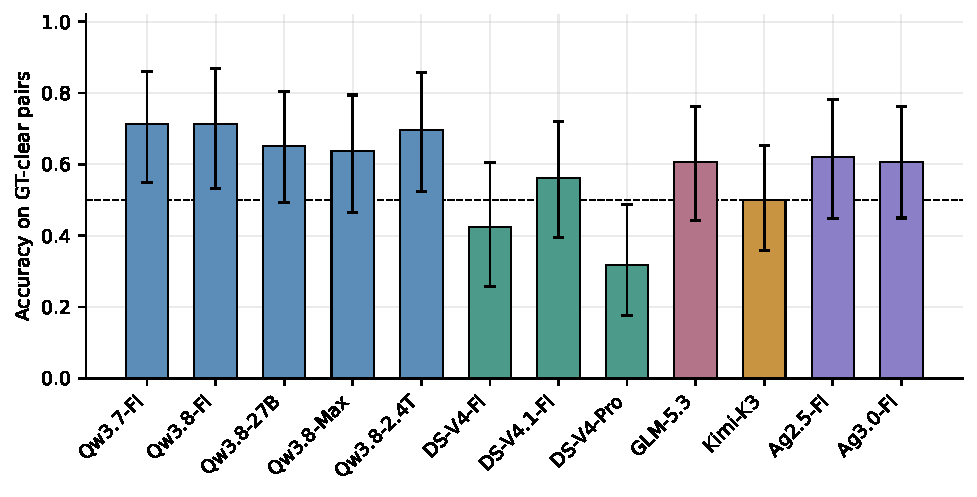
\includegraphics[width=0.72\textwidth]{figures/fig_accuracy.pdf}
\caption{Ground-truth accuracy on the 66 ground-truth-clear pairs
(canonical order), with question-level cluster bootstrap 95\% CIs. The
dashed line marks chance. The proprietary Agnes references are shown in
purple.}
\label{fig:accuracy}
\end{figure}

\begin{figure}[t]
\centering
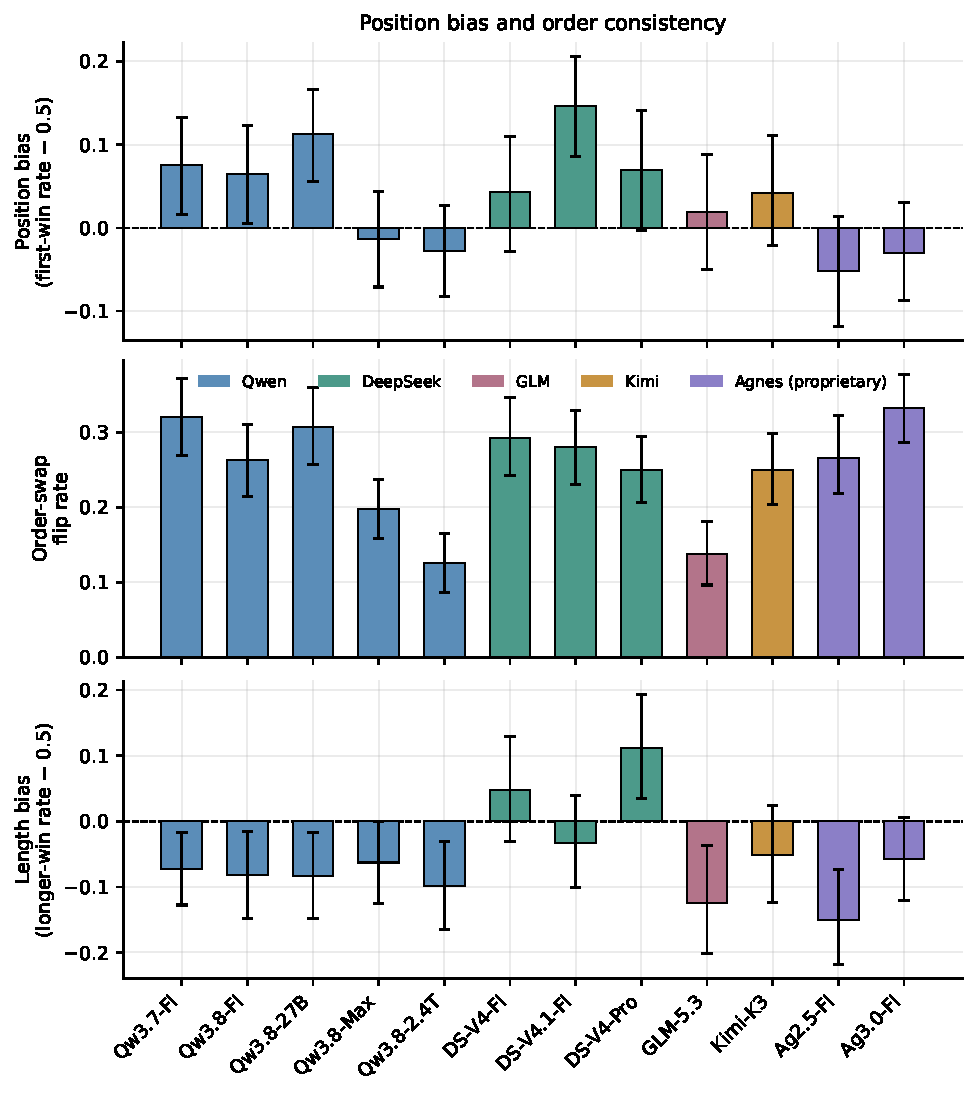
\includegraphics[width=0.78\textwidth]{figures/fig_bias.pdf}
\caption{Bias trio per judge with 95\% CIs: position bias (top), order-swap
flip rate (middle), and length bias (bottom). Dashed lines mark the
unbiased null.}
\label{fig:bias}
\end{figure}

\begin{figure}[t]
\centering
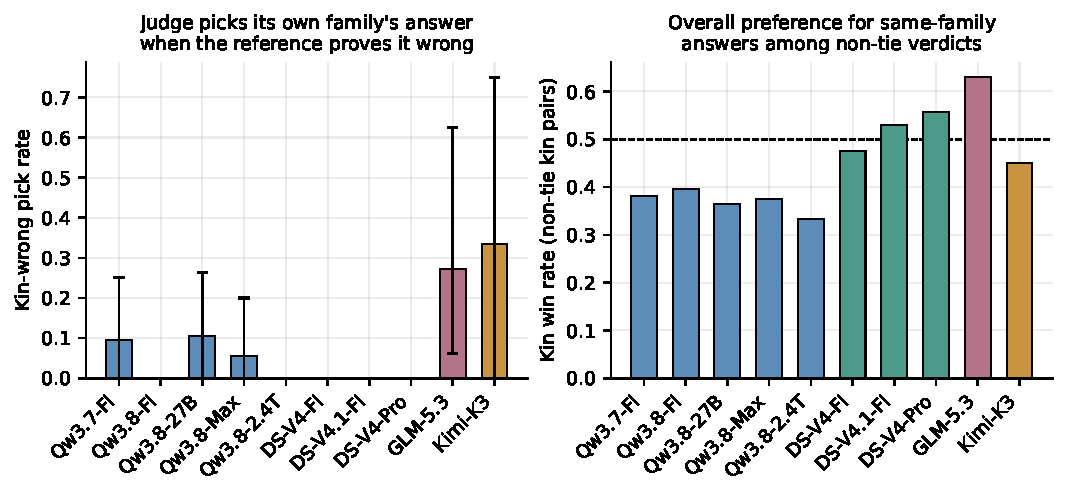
\includegraphics[width=0.9\textwidth]{figures/fig_kin.pdf}
\caption{Family preference for the ten open judges. Left: kin-wrong pick
rate, the fraction of ground-truth-clear kin pairs in which the judge picks
its own family's answer although the reference proves it wrong. Right:
overall kin win rate among non-tie kin pairs (dashed line: 0.5).}
\label{fig:kin}
\end{figure}

\begin{figure}[t]
\centering
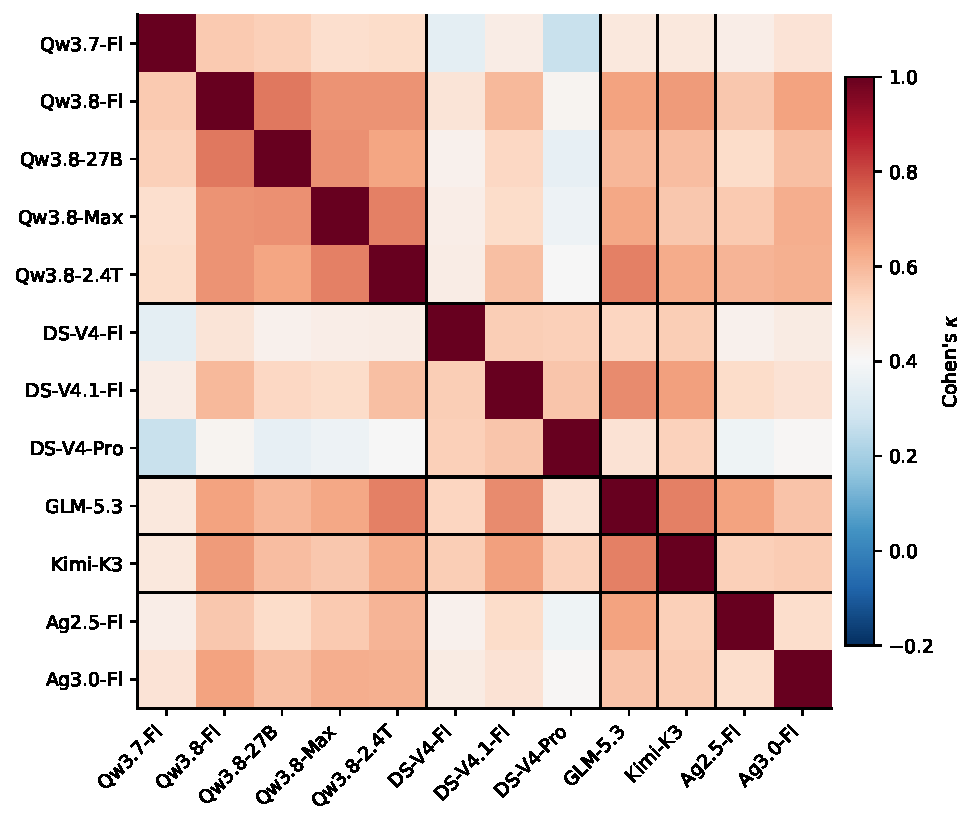
\includegraphics[width=0.7\textwidth]{figures/fig_agreement.pdf}
\caption{Pairwise Cohen's kappa between judges on canonical-order verdicts.
Black grid lines separate model families.}
\label{fig:agreement}
\end{figure}

\begin{figure}[t]
\centering
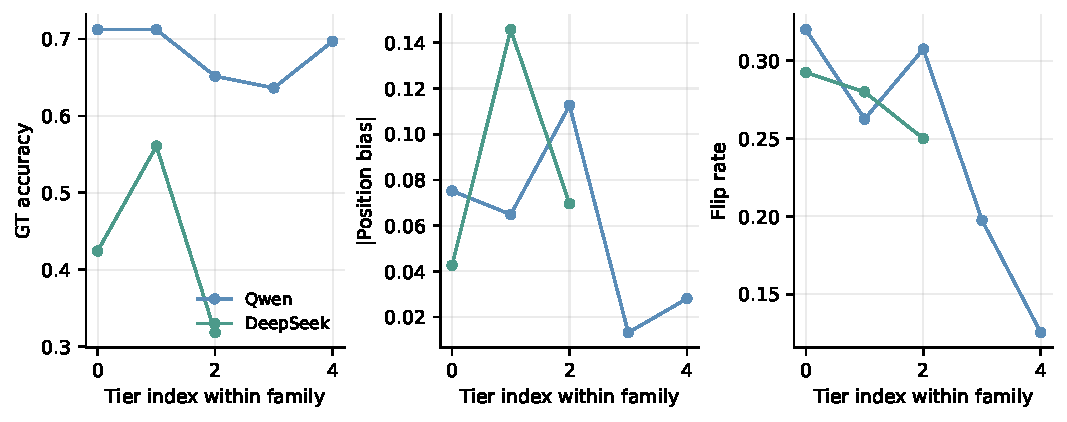
\includegraphics[width=0.95\textwidth]{figures/fig_scale.pdf}
\caption{Within-family trends across capability tiers for families with at
least two tiers: ground-truth accuracy (left), absolute position bias
(middle), and order-swap flip rate (right).}
\label{fig:scale}
\end{figure}

\begin{figure}[t]
\centering
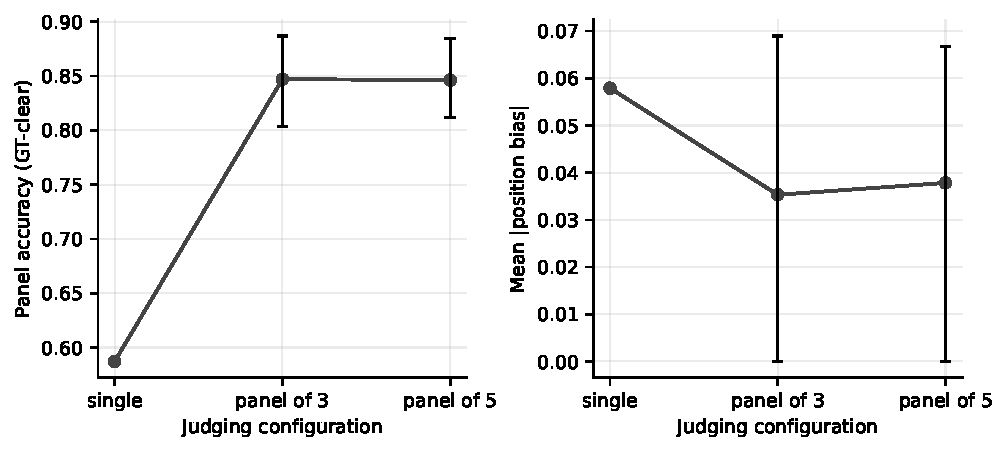
\includegraphics[width=0.85\textwidth]{figures/fig_panel.pdf}
\caption{Majority-vote panels of open judges: ground-truth accuracy (left)
and mean position bias (right) for single judges and panels of three and
five. Panels raise accuracy but pass the shared position component
through essentially unchanged.}
\label{fig:panel}
\end{figure}

The audit yields one message above all: \emph{free judges are usable, but
only after screening, and never naively}. The properties that matter most
are not the ones model cards advertise. Parameter count and flagship status
predict neither accuracy nor severity; the DeepSeek Pro flagship is the
least useful judge in the roster precisely because it abstains on most
pairs, while a small flash checkpoint from the same provider discriminates
better. What predicts behaviour is a combination of provider-level tuning
(severity), instruction sensitivity (length), lineage (kinship), and
deployment configuration (thinking mode for order stability). We distill
the findings into six guidelines for zero-cost judging.

\paragraph{G1: Screen for severity collapse first.}
Before deploying any free judge, run a twenty-pair probe with a known
quality difference and measure the tie rate. A judge that ties on more than
about 40\% of clearly-different pairs (as the DeepSeek checkpoints,
GLM-5.3, Kimi-K3, and one of the two proprietary references do here) will
undermine any downstream use that assumes discrimination---leaderboards,
win-rate estimation, best-of-$n$ selection---regardless of how sound its
individual verdicts are. Severity is the cheapest possible screen: it
requires no ground truth, only variation.

\paragraph{G2: Prefer Qwen mid and flagship tiers as workhorses.}
Within this roster, Qwen3.8-27B, Qwen3.8-Max, and Qwen3.8-2.4T offer the
best combination of accuracy (0.64--0.70), moderate severity (tie rates
0.24--0.31), and order stability (flip rates 0.13--0.31). The 2.4T
flagship, served with mandatory reasoning, is the single most
order-stable judge and shows no measurable position bias, at the cost of
roughly double the token consumption of the flash tiers.

\paragraph{G3: Keep order swapping; add panel position balancing.}
Even the most order-stable judge flips on one pair in eight, and the least
stable on one in three. Order swapping remains mandatory. Our panel results
add a subtler warning: majority voting over judges passes the \emph{shared}
position component through essentially unchanged (mean bias $+0.04$ for
panels versus $+0.04$ for singles on the same pair set), so panels should
aggregate over order-swapped
judgements---for example by judging each pair in both orders and requiring
the majority to agree on the canonical verdict---rather than over raw
single-order verdicts.

\paragraph{G4: Soften the anti-verbosity instruction.}
The standard ``do not reward length'' sentence overshoots into measurable
short-answer preference ($-0.46$ log-odds per 1{,}000 characters). Either
soften it to ``length alone does not determine quality'', or standardise
candidate lengths before comparison, and re-check length bias after any
prompt change with a length-stratified probe.

\paragraph{G5: Audit kinship with ground truth before trusting a judge on
its own ecosystem.}
Family preference is real but lineage-specific: the Qwen judges
significantly avoid their own family's answers, while GLM-5.3 and Kimi-K3
reward theirs even when the reference proves the kin answer wrong (27--33\%
kin-wrong pick rate on small samples). Any evaluation that uses a judge
from family $X$ to rank models that include family $X$ should run a
ground-truth-controlled kin probe first; the entire probe costs a few
hundred free-tier tokens.

\paragraph{G6: Build panels across families, not across tiers.}
Agreement structure shows family-level fault lines (Qwen--DeepSeek mean
$\kappa=0.44$), so a three-judge panel drawn from three families decorrelates
errors far more effectively than three tiers of the same family. A panel of
three open judges reaches 0.85 accuracy on
ground-truth-clear pairs---better than the best single free judge (0.71)
and statistically indistinguishable from panels that include proprietary
references (0.85)---at zero monetary cost.

\paragraph{Relation to prior work.}
Our findings refine three strands of the literature. The verbosity-bias
literature documents that judges favour longer answers; we show that the
standard mitigation instruction flips the sign of the effect, a
prompt-sensitivity phenomenon that length-controlled win rates do not
capture. The self-preference literature establishes that judges recognise
and reward their own generations; we generalise the unit of analysis from
model to family and show that the effect's \emph{direction} varies by
lineage, which matters for the increasingly common situation where one
provider both ships the judge and supplies some of the candidates. Finally,
panel proposals argue that judge diversity averages away idiosyncratic
errors; our panel analysis refines this: diversity cancels the independent
noise component strongly enough to lift accuracy markedly, but the shared
position component passes through majority voting unchanged, so panels must
still pair diversity with order-balanced aggregation.

%% ==================================================================
\section{Limitations}
\label{sec:limitations}

Our findings should be read against several limitations. First, the ten
open-source judges are all served through a single provider endpoint, and the
two proprietary judges through a second one. Although this removes serving
differences as a confound within each group, it also means that our
observations reflect the providers' quantization and serving configurations
of each checkpoint rather than the raw open weights, and replication on
self-hosted inference may differ in detail; in particular, the Agnes platform
injects undisclosed system instructions ahead of our judging prompt, so the
proprietary judges' absolute numbers are indicative rather than strictly
comparable to the open panel. Second, the roster covers four
model families that all originate from Chinese development teams, because
these are the families with usable free tiers on the chosen platform at the
time of the study; Western open families such as Llama or Mistral were not
available under the zero-cost constraint, so our family-preference findings
should be generalized to those families with care, and the GLM family is
represented by a single checkpoint, so GLM-specific conclusions rest on one
observation. Third, two judges are
served with a mandatory reasoning phase, which is entangled with their
family identity and tier; we treat thinking mode as an observational
variable and report where it plausibly matters, but a fully crossed
thinking-by-family design is not realizable on this platform. Fourth, the
evaluation uses 400 pairs over four English-language domains. While the
stratified design gives every judge the same stimulus set and the bootstrap
accounts for question-level clustering, the absolute number of
ground-truth-clear kin pairs per family remains modest, and kin-preference
estimates for individual judges carry correspondingly wide intervals. Fifth,
our generators produce single answers per question at a moderate sampling
temperature; verdicts could vary with additional samples, and we leave
multi-sample generation to future work. Finally, the two open-ended domains
lack ground truth, so for those domains our reliability claims are about
agreement among judges rather than closeness to correctness.

%% ==================================================================
\section{Conclusion}
\label{sec:conclusion}

We audited the judging behaviour of every LLM reachable at zero monetary
cost on two public platforms at the time of study: ten open-source judges
from four families and two proprietary free-tier references, evaluated
under one protocol over 400 answer pairs in four domains, with both
presentation orders, a test--retest subset, and ground-truth-controlled
family-preference probes. The picture that emerges is nuanced but
actionable. Free judges are viable: the strongest open checkpoints reach
0.71 accuracy on verifiable pairs and inter-judge agreement comparable to
published commercial audits, and a three-judge cross-family panel of free
models beats the best single free judge. But viability is conditional on
screening, because the failure modes are systematic rather than random:
severity collapse that silences entire families, an anti-verbosity
instruction that overshoots into short-answer preference, lineage-specific
kin favouritism---within the four families studied---that survives
ground-truth control, and majority voting that inherits, rather than
removes, the shared position bias. Every one
of these failure modes is detectable with probes that cost a few hundred
tokens, and every probe ships with the released artifact, so the audit
and its screening kit can be re-run by any group as free-tier catalogues
evolve. As evaluation infrastructure comes to rest on machine judgement,
the reliability of the judges themselves---especially the ones that cost
nothing---deserves the same systematic attention that has been lavished on
the systems they grade.

%% ==================================================================
\section*{Data and Code Availability}

All prompts, the 200-question evaluation set, raw verdict logs, and analysis
scripts are released at
\texttt{github.com/43aquarius/LLM-as-a-Judge}.

\section*{Acknowledgements}

%%ACK-PLACEHOLDER%%

\bibliography{refs}

\end{document}
